\section{Bemeneti példányok}\label{sec:BENCHMARK-PROBLEM-INSTANCES}
Benchmark tesztelés végett a \citeN{ventresca2012global} által javasolt gráfhalmazt fogjuk használni, amelyben négy alapvető típus jelenik meg, mindegyik a maga jellegzetességeivel.
A következőkben ezeket a modelleket szeretnénk röviden ismertetni.


\subsection{Barabási–Albert modell}



\subsection{Erdős–Rényi modell}



\subsection{Forest-fire modell}



\subsection{Watts–Strogatz modell}



\begin{figure}[ht]
  \begin{subfigure}[b]{0.5\linewidth}
    \centering
    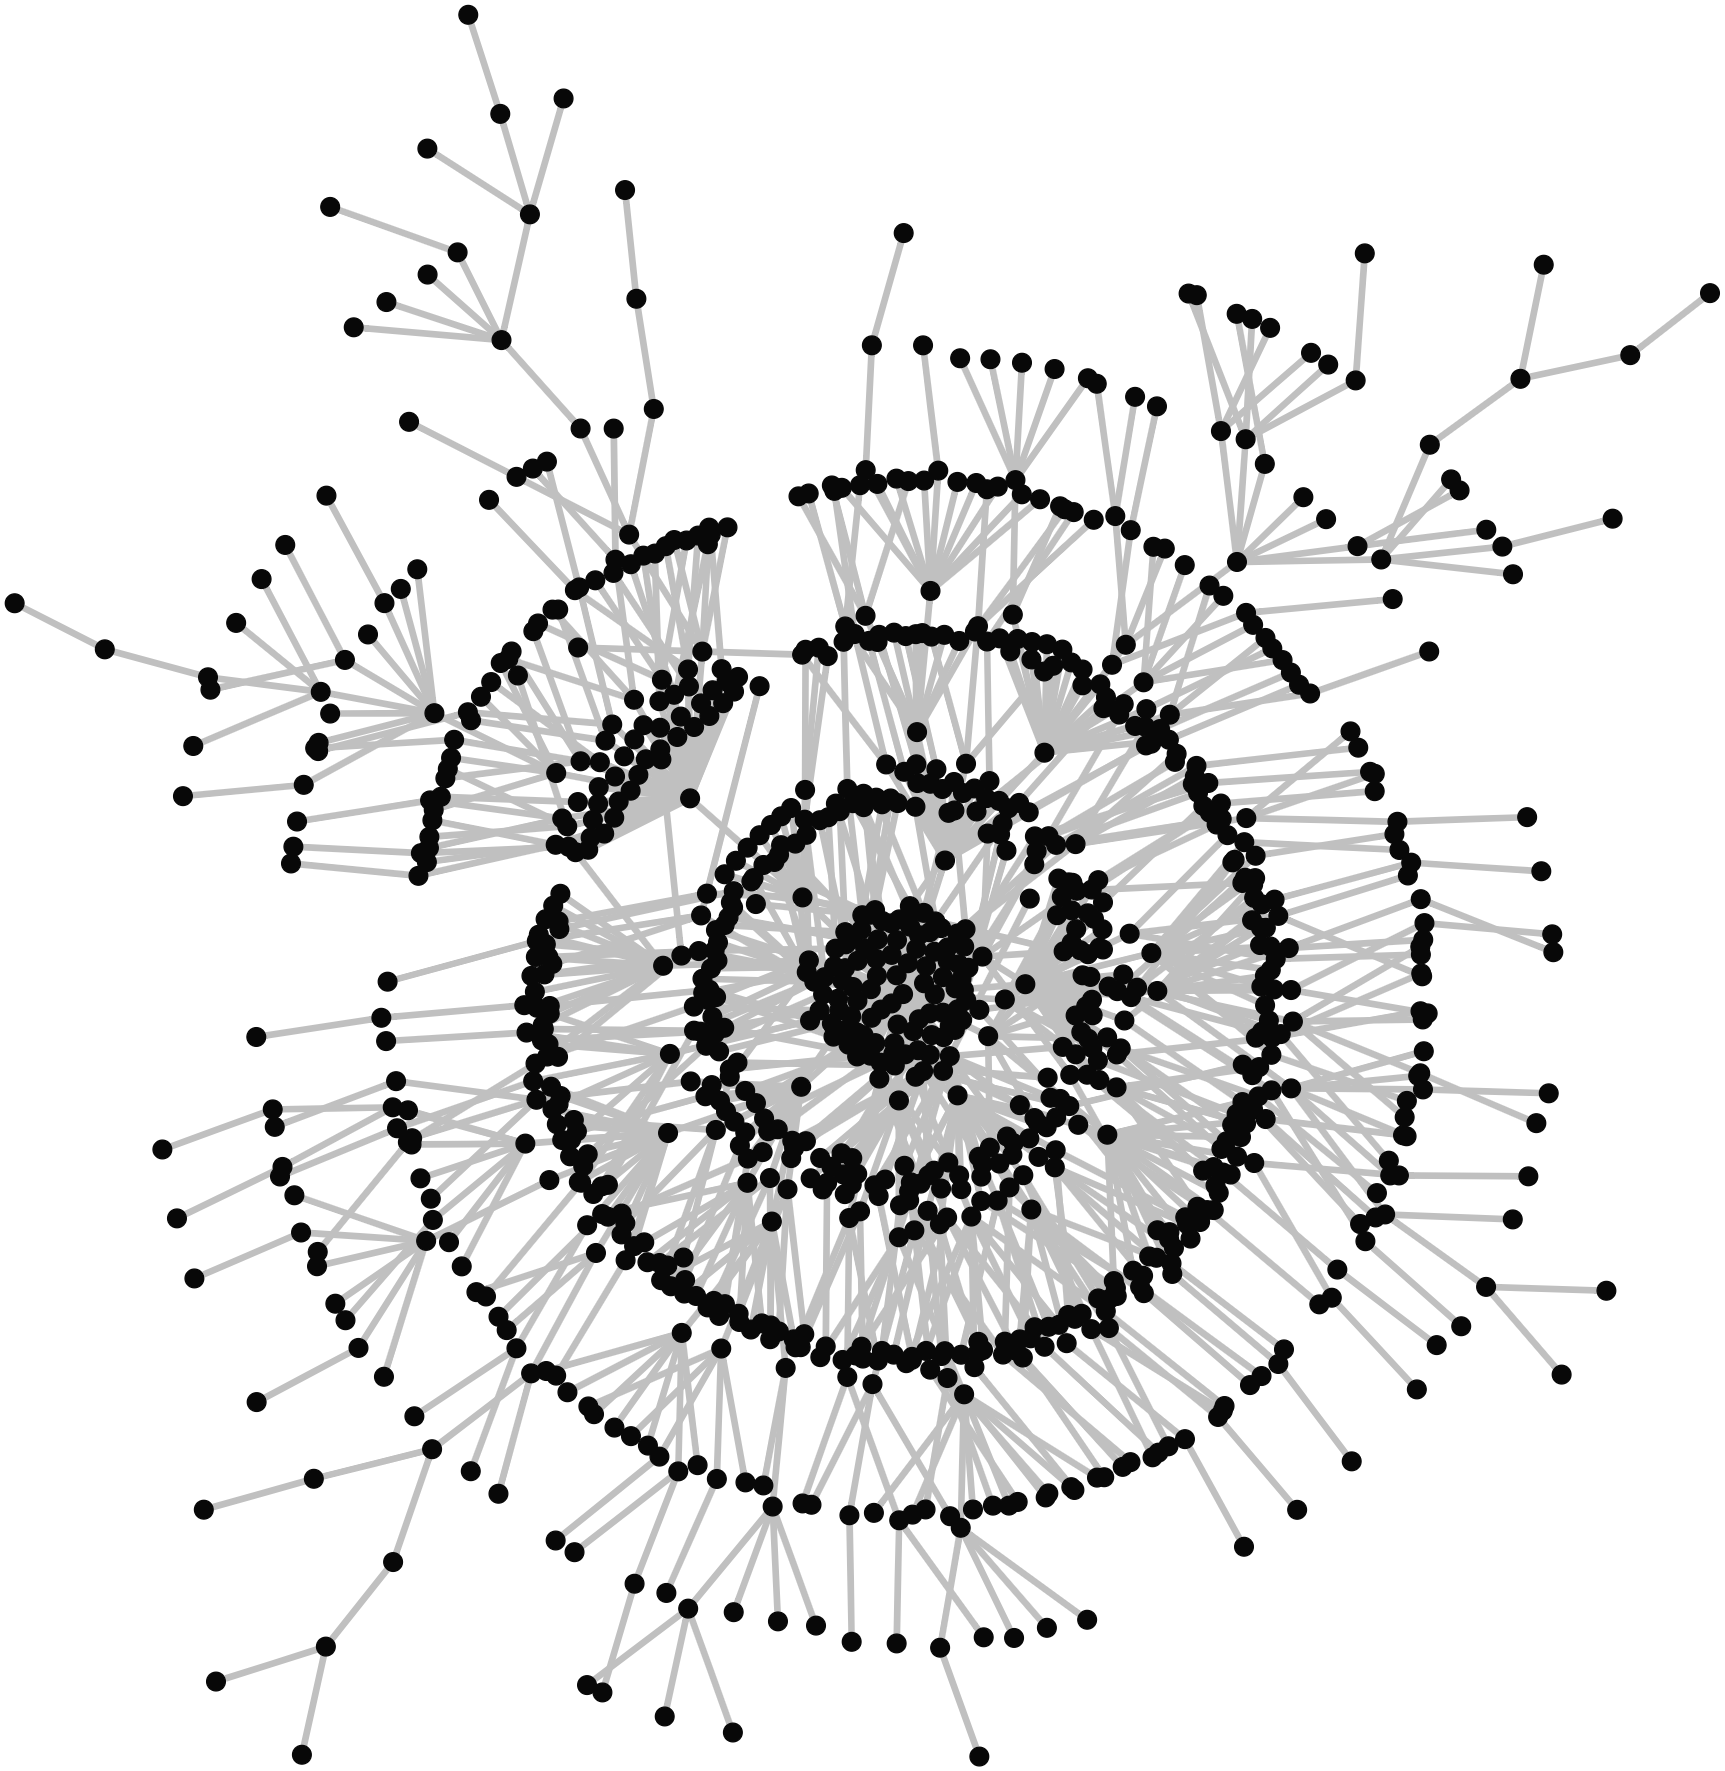
\includegraphics[width=1\linewidth]{images/barabasi_albert_model.png}
    \caption{ Barabási–Albert típusú gráf, 1000 csomópont. }
    \label{fig:BARABASI_ALBERT_MODEL}
    \vspace{4ex}
  \end{subfigure}%%
  \begin{subfigure}[b]{0.5\linewidth}
    \centering
    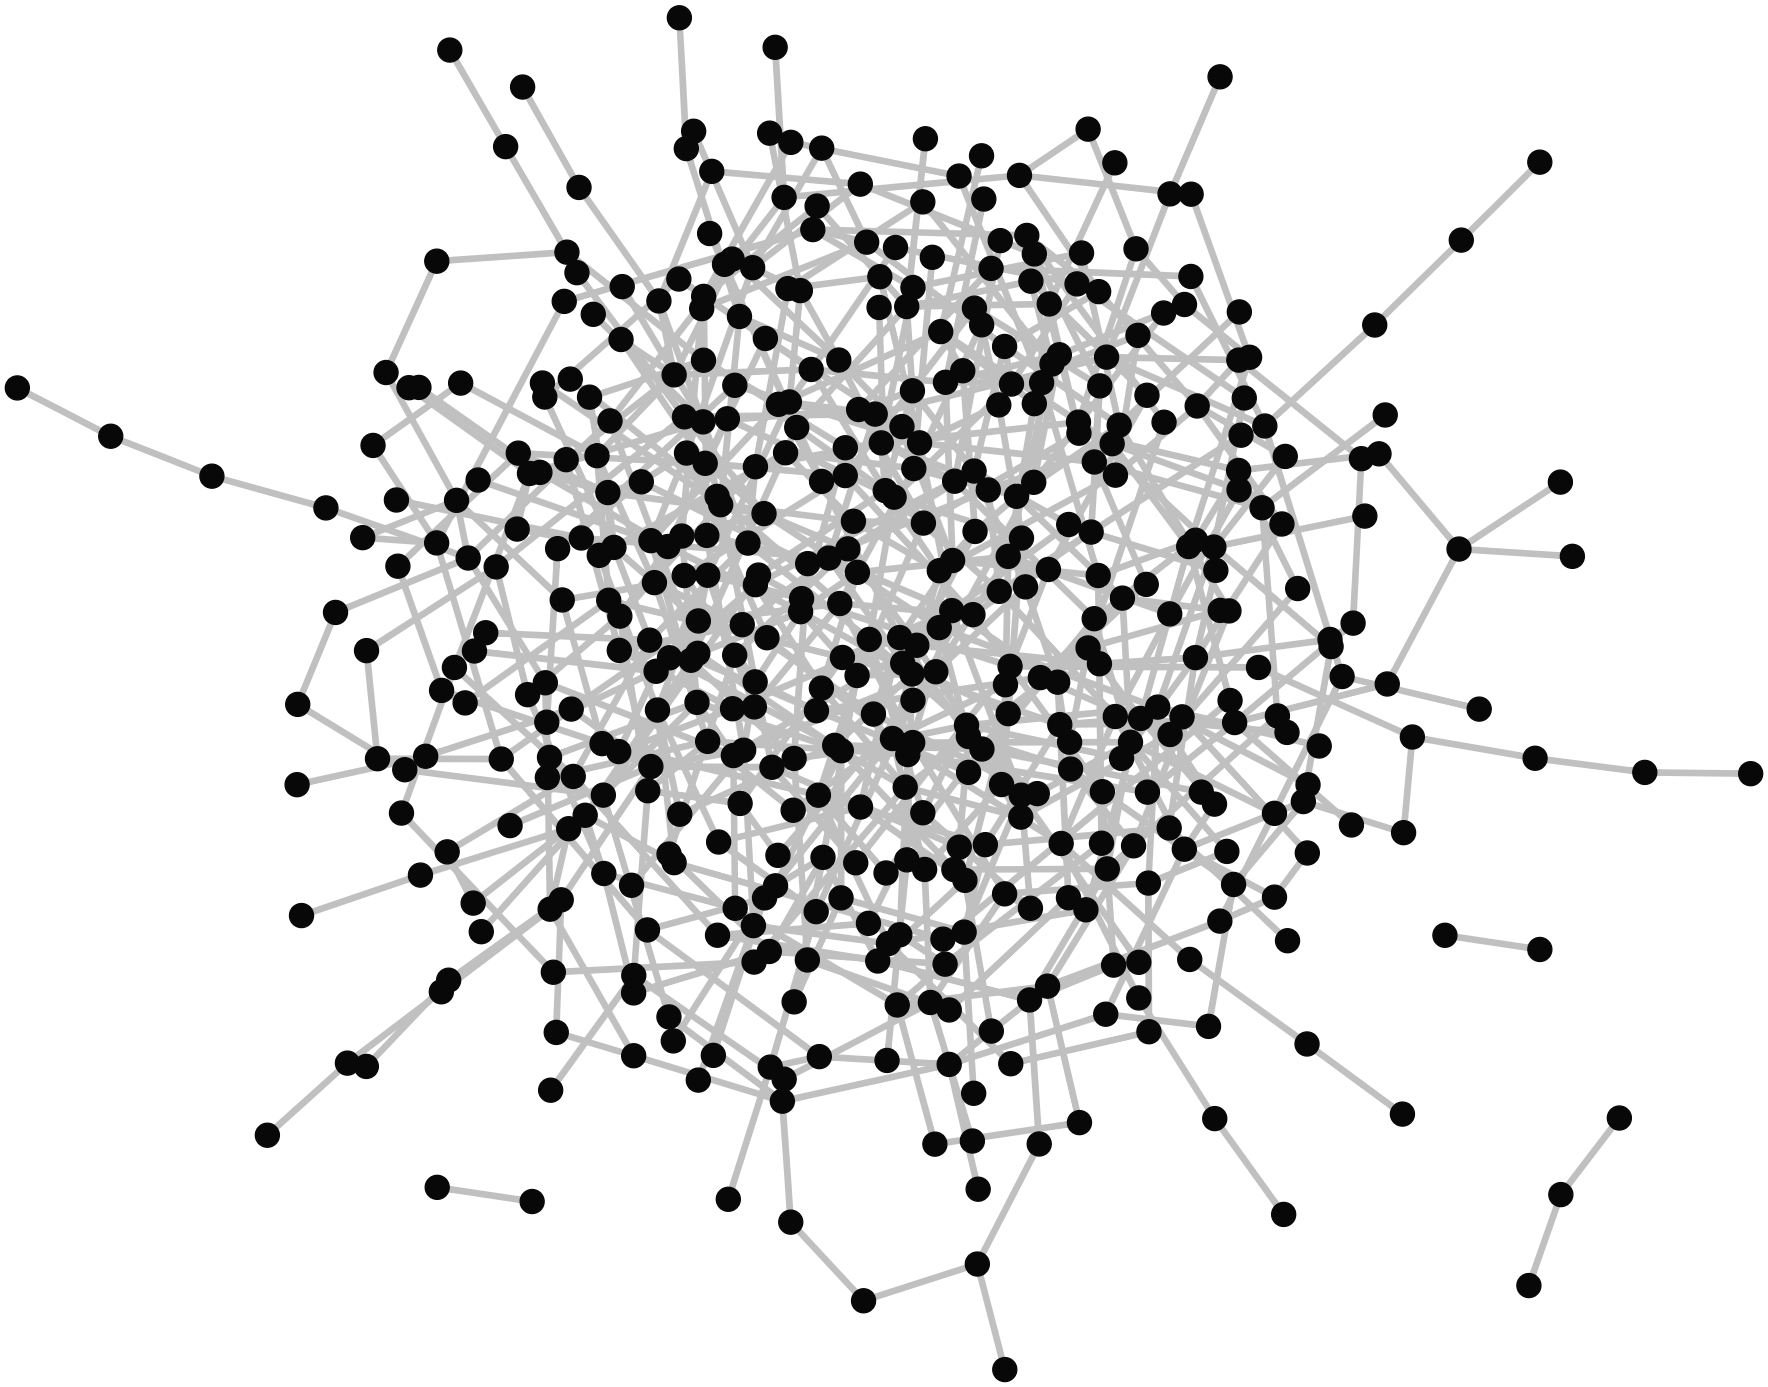
\includegraphics[width=1\linewidth]{images/erdos_renyi_model.png}
    \caption{ Erdős–Rényi típusú gráf, 466 csomópont. }
    \label{fig:ERDOS_RENYI_MODEL}
    \vspace{4ex}
  \end{subfigure}
  \begin{subfigure}[b]{0.5\linewidth}
    \centering
    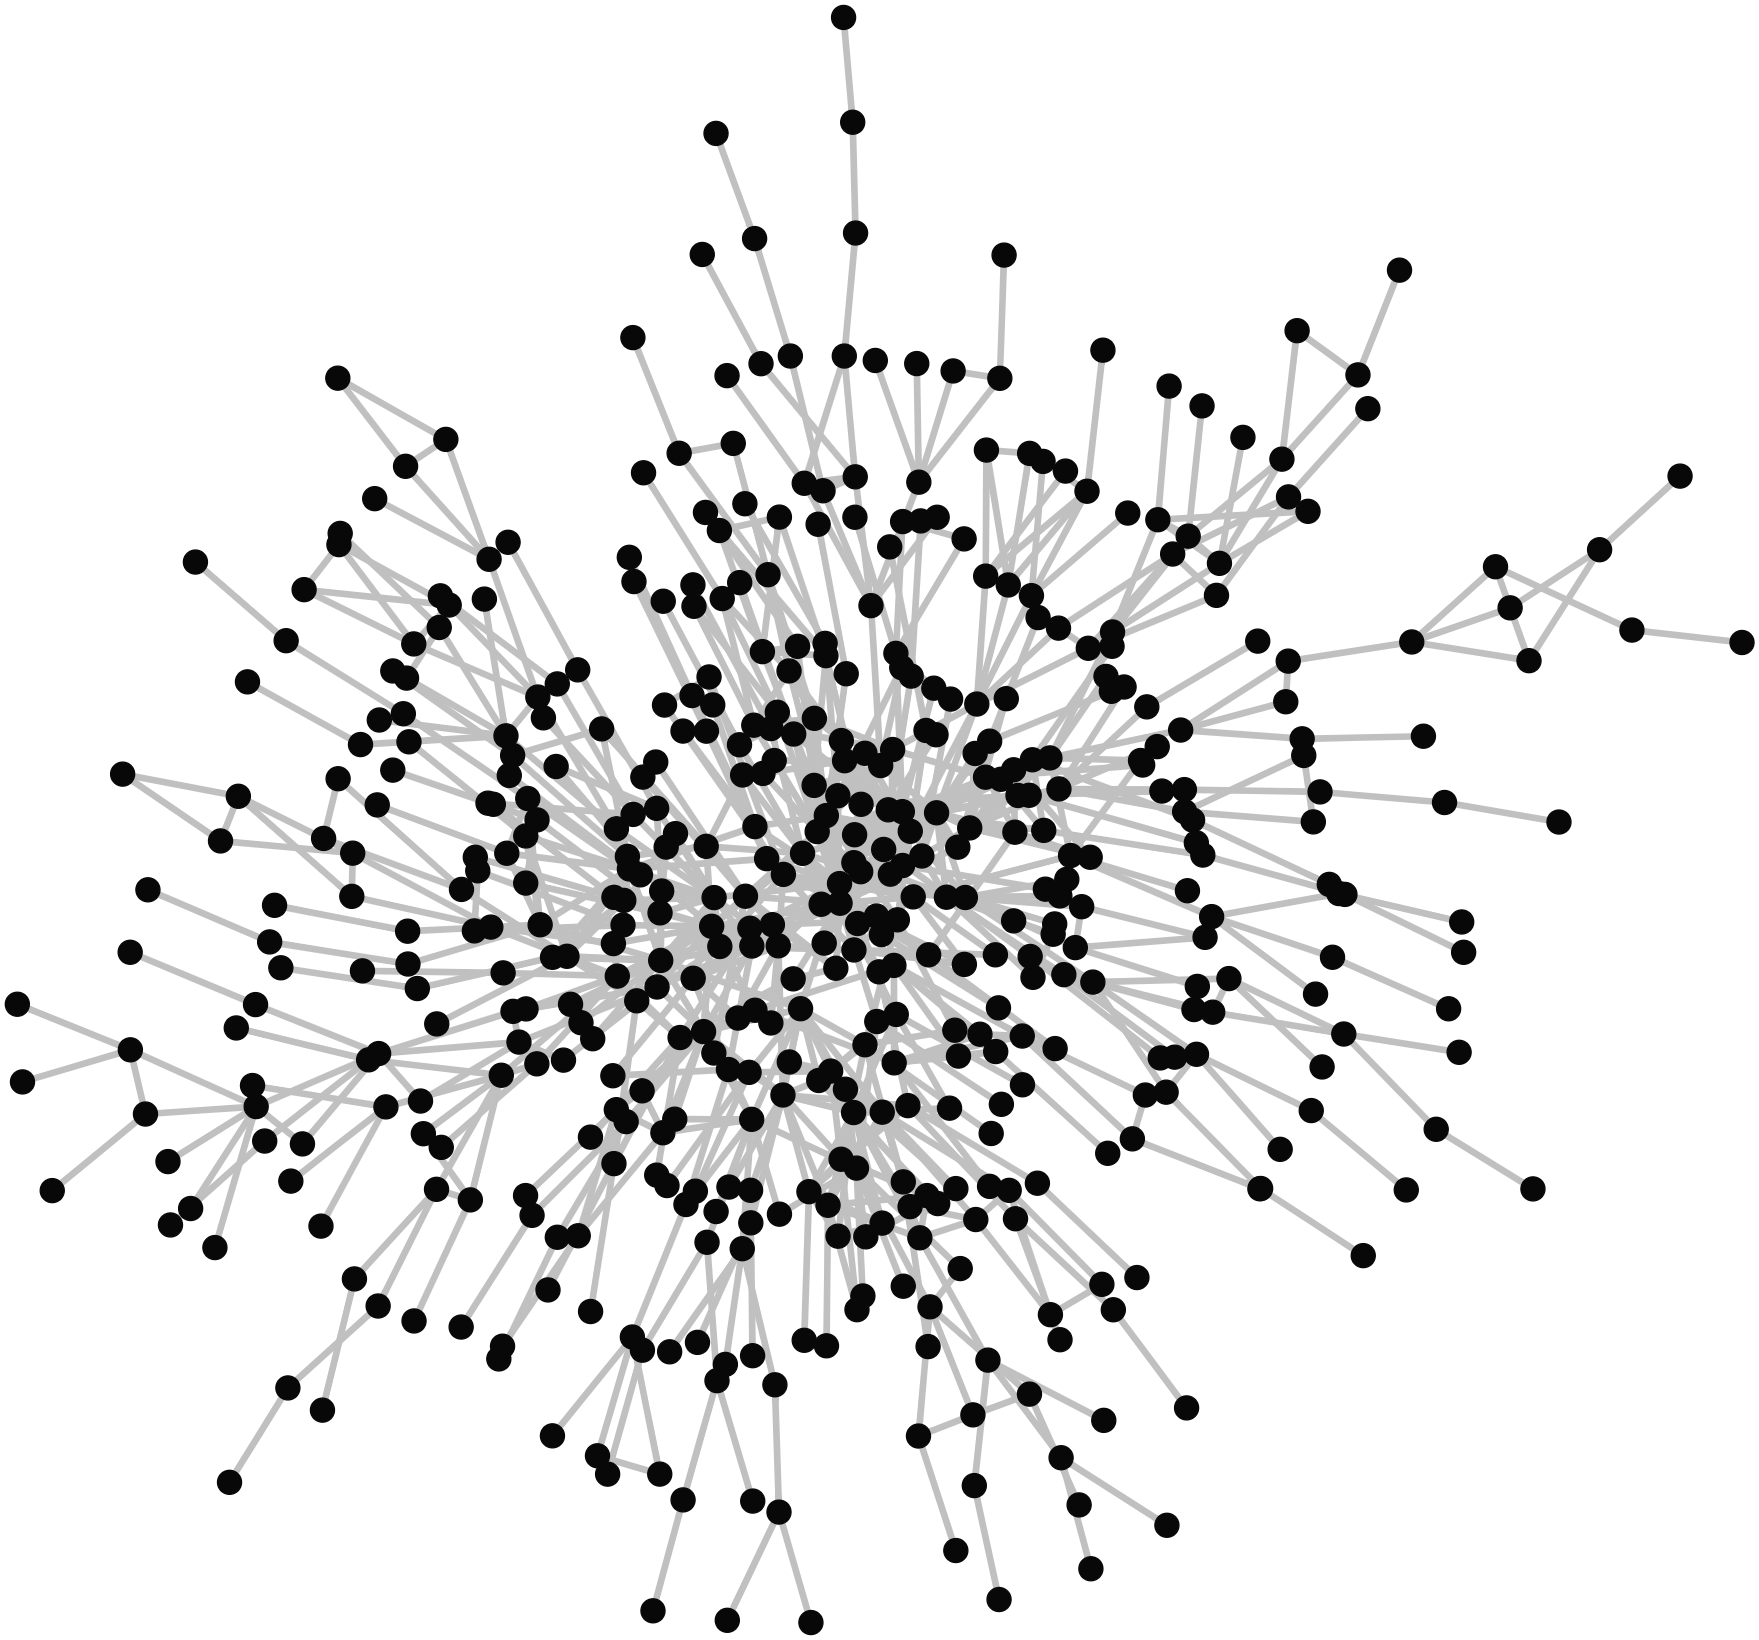
\includegraphics[width=1.15\linewidth]{images/forest_fire_model.png}
    \caption{ Forest-fire típusú gráf, 500 csomópont. }
    \label{fig:FOREST_FIRE_MODEL}
  \end{subfigure}%%
  \begin{subfigure}[b]{0.5\linewidth}
    \centering
    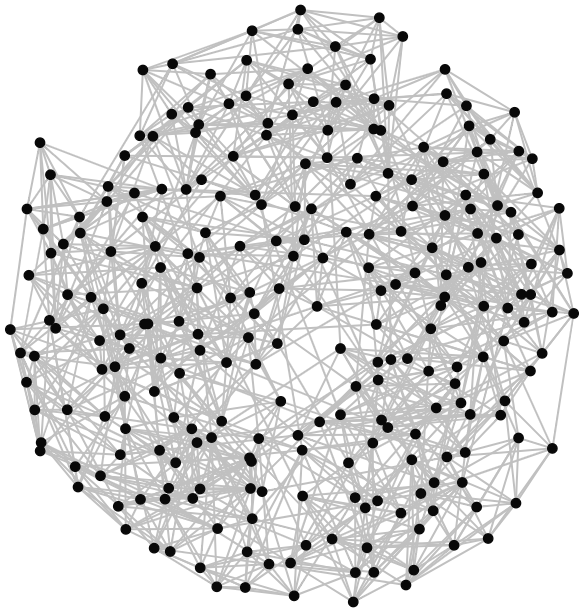
\includegraphics[width=0.85\linewidth]{images/watts_strogatz_model.png}
    \caption{ Watts–Strogatz típusú gráf, 500 csomópont. }
    \label{fig:WATTS_STROGATZ_MODEL}
  \end{subfigure}\\
  \caption{A bemeneti példányok négy különböző modellje.}
  \label{fig:BENCHMARK_INSTANCES}
\end{figure}
